\section{Вступление}

Компьютерное зрение - это наука, занимающаяся разработкой алгоритмов
и систем для анализа и интерпретации изображений, созданных с помощью
камер и других датчиков. Одной из ключевых проблем компьютерного
зрения является восстановление трехмерной формы объектов
из двумерных изображений. Для решения этой проблемы используется
много различных технологий, одной из которой является
фотометрическое стерео.

Фотометрическое стерео - это метод восстановления трехмерной формы
объектов из серии изображений, полученных под различными углами
освещения. Он основан на анализе освещения объекта,
что позволяет получать данные о его форме. Суть метода заключается
в анализе изменений яркости поверхности объекта в различных точках
изображения при разных углах освещения. На основе этих данных
можно получить трехмерную модель поверхности объекта.

\begin{figure}[h]
  \centering
  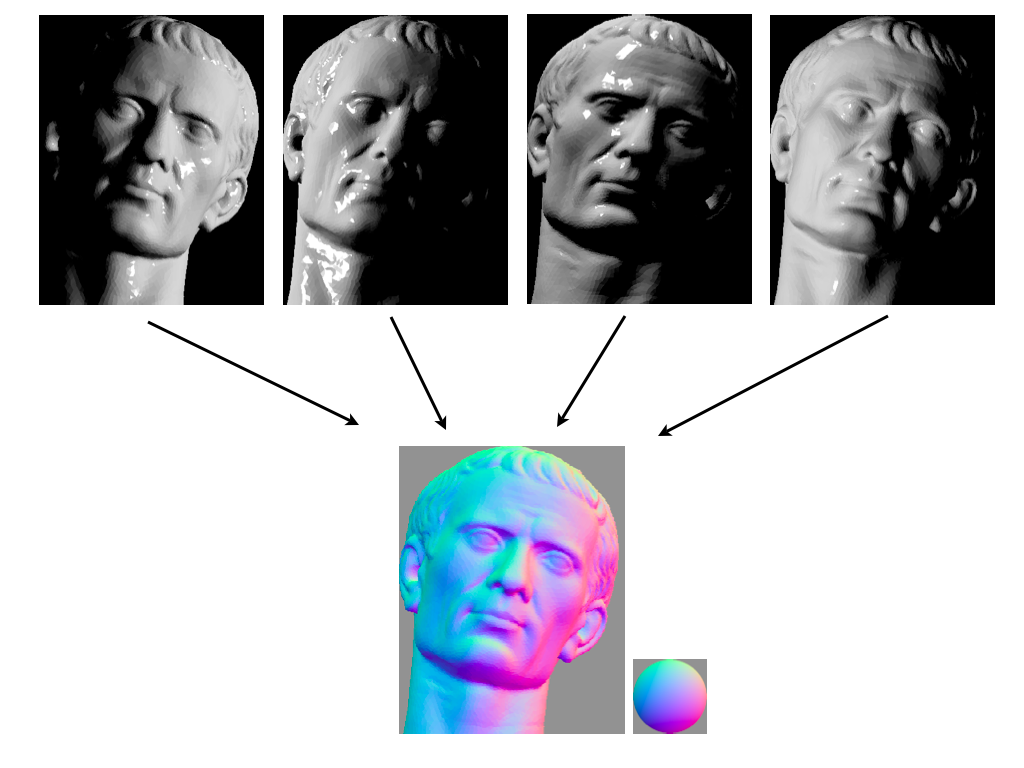
\includegraphics[scale=0.3]{tex/example.png}
\end{figure}

Один из ключевых элементов фотометрического стерео - это модель отражения
света, которая описывает изменение яркости той же точки при
изменении направления освещения. В случае модели Ламберта
изменения яркости точки отображают только нормаль поверхности,
и при этом яркость точки не зависит от направления освещения.
Это свойство значительно упрощает процесс восстановления поверхности,
поскольку можно точно определить нормали по изображениям под
разными углами.

Фотометрическое стерео может быть использовано в различных
областях приложений, таких как инспекция качества
промышленных изделий, создание 3D-моделей для игр и виртуальной
реальности и многого другого. Но несмотря на все его
преимущества, метод фотометрического стерео довольно сложен
и чувствителен к шумам и погрешностям, таким как тени,
блики и т.д.

В данной курсовой работе мы рассмотрим основные принципы, которые
лежат в основе фотометрического стерео, а также алгоритм
восстановления поверхности объектов из полученных нормалей.
В конце мы проанализируем различные ограничения и сложности,
связанные с применением этого метода.
